\documentclass{article} % For LaTeX2e
\usepackage{final_project,times}
\usepackage{hyperref}
\usepackage{tikz}
\usepackage{float}
\usepackage{graphicx}
\usepackage{caption}
\usepackage{subcaption}
\usetikzlibrary{graphs,graphs.standard}

%\documentstyle[nips12submit_09,times,art10]{article} % For LaTeX 2.09


\newtheorem{theo}{Theorem}
\newtheorem{ax}{Axiom}
\newtheorem{lemma}{Lemma}
\newtheorem{claim}{Claim}
\newtheorem{prop}{Proposition}
\newtheorem{cor}{Corollary}
\newtheorem{defi}{Definition}
\newtheorem{rem}{Remark}
\newtheorem{ex}{Exercise}
\newtheorem{ob}{Observation}
\newtheorem{as}{Assumption}

\title{Legislation approval ratings prediction via vote correlation}


\author{
Yuan Deng, Junyang Gao, Xiaoxue Wang \\
Department of Computer Science\\
Duke University\\
\texttt{\{ericdy, jygao, xxw211\}@cs.duke.edu} \\
}

\newcommand{\fix}{\marginpar{FIX}}
\newcommand{\new}{\marginpar{NEW}}

\nipsfinalcopy

\begin{document}


\maketitle

\begin{abstract}
We implement the machine learning techniques, including topic modeling, support vector classification, and spectral partitioning, to predict the legislation approval ratings. Our novelty is to incorporate a new feature called \textbf{vote correlation}, which represents the voting similarities / correlations between two voters. 
\end{abstract}

\section{Introduction}
    In United States, there exists a special process to turn a bill into a law, including\cite{billToLaw}
    \begin{itemize}
        \item Introducing the Bill and Referral to a Committee
        \item Committee Action: Hearings and Mark Up
        \item Committee Report
        \item Floor Debate and Votes
        \item Referral to the Other Chamber
        \item Conference on a bill
        \item Action by the President
        \item Overriding a Veto
    \end{itemize}
    Intuitively, to turn a bill into a law, there are several rounds of votes to decide whether the clauses or properties of the bills are acceptable or not. We focus on the votes, the ``floor debate and votes'' sub-process, to predict the voting  results. In order to predict results, one straightforward way is to predict each voter's vote according to their voting history and aggregate their votes to form an outcome. However, we attempt another way to formulate the problem and introduce a new concept, called {\em vote correlation} to make use of the second order information in order to improve our prediction.

\section{Related work}

Related works in the similar topic was done by Yano, Smith and Wilkerson\cite{textual} and Zach Cain, Pamela Chua and Kristian Gampong\cite{stanford}. Yano\cite{textual} mainly focused on exploring textual features on legislation bill/vote to predict its survival in Congressional committees. While Zach\cite{stanford} learned from individual voter's voting record to make the prediction. In our project, besides exploring textual features on legislation bill/vote, we will use vote correlation between each pair of congressmen. Our new prediction model and methodology differs significantly from their work. Our experiment result (Section 6) has shown that our prediction model can achieve a high accuracy.

\section{Outline of our algorithm}
Different from the traditional way of prediction, in which based on the voting history of each voter, the system simply predicts the vote for the new legislation, our system works as follows:     
    \begin{enumerate}         
        \item For each pair of voters, compute vote correlations;
        \item Classify voters into two groups by vote correlations;
        \item Predict the aggregate vote of the two groups;
    \end{enumerate}

\begin{figure}
\centering
\begin{subfigure}{.5\textwidth}
  \centering
  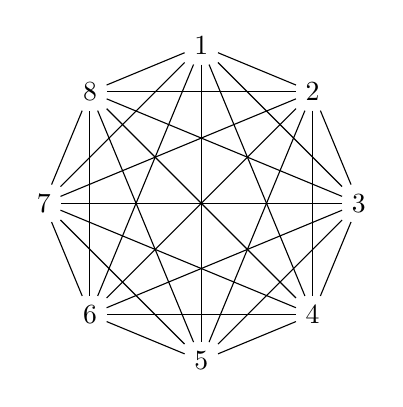
\begin{tikzpicture}
  \graph { subgraph K_n [n=8,clockwise,radius=2cm] };
  \end{tikzpicture}
  \caption{compute all-pair vote correlation/similarities}
  \label{fig:sub1}
\end{subfigure}%
\begin{subfigure}{.5\textwidth}
  \centering
  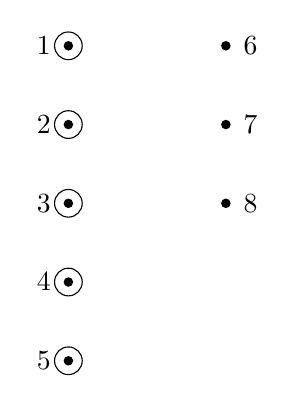
\begin{tikzpicture}
    [
        main node/.style={circle, draw, inner sep=0pt, minimum width=3pt, fill=black}
    ]

    \node [main node] (1) at (-1, 2.5) {};
    \node [main node] (2) at (1, 2.5) {};
    \node [main node] (3) at (-1, 1.5) {};
    \node [main node] (4) at (1, 1.5) {};
    \node [main node] (7) at (-1, -0.5) {};
    \node [main node] (8) at (-1, -1.5) {};
    \node [main node] (5) at (-1, 0.5) {};
    \node [main node] (6) at (1, 0.5) {};

    \draw (-1.1, 2.5) node[left] {$1$};
    \draw (1.1, 2.5) node[right] {$6$};
    \draw (-1.1, 1.5) node[left] {$2$};
    \draw (1.1, 1.5) node[right] {$7$};
    \draw (-1.1, 0.5) node[left] {$3$};
    \draw (1.1, 0.5) node[right] {$8$};
    \draw (-1.1, -0.5) node[left] {$4$};
    \draw (-1.1, -1.5) node[left] {$5$};


    \draw (-1, 2.5) circle (5pt);
    \draw (-1, 1.5) circle (5pt);
    \draw (-1, 0.5) circle (5pt);
    \draw (-1, -0.5) circle (5pt);
    \draw (-1, -1.5) circle (5pt);
    \end{tikzpicture}
    
  \caption{Partition voters into two groups according to their vote correlation matrix.}
  \label{fig:sub2}
\end{subfigure}
\caption{An example of legislation approval rating prediction process with 8 voters}
\label{fig:test}
\end{figure}
 

\section{Problem Formulation}
    Assume the set of bills is $\mathcal B$ while the set of votes are $\mathcal V$. Moreover, each vote is corresponding to a bill, and thus, we denote $\mathcal V_b \subseteq \mathcal V$ as the set of votes corresponding to a specific bill $b \in \mathcal B$. Let $F_b$ and $F_v$ represents the feature vector of bill $b \in \mathcal B$ and $v \in \mathcal V$, respectively. In addition, we concatenate the two feature vector to get the real feature vector of a vote, which is $G_v = F_v \circ F_b$.
    
    As for the voters, suppose the set of voters is $\mathcal N$ and each voter $p \in \mathcal N$ participates into set of votes $\mathcal V_p$. On the contrary, denote $\mathcal N_v$ for $v \in \mathcal V$ to be the set of voters participating in vote $v$. 
    
    Define function $f_p: \mathcal V_p \to \{0,1\}$ as the function mapping the vote $v \in \mathcal V_p$ to his vote, which is either {\em yes}(1) or {\em no}(0). We introduce the notion of {\em vote correlation} for vote $v \in \mathcal V$ as a function $g_v: \mathcal N_v \times \mathcal N_v \to \{0, 1\}$ to represent whether two voters have the same vote for a specific vote $v$.
    
    Finally, according to the function $g_v$ for $v \in \mathcal V$, we divide the voters into two groups by a function $D_v : (g_v: \mathcal N_v \times \mathcal N_v \to \{0, 1\}) \to \{0, 1\}^{|\mathcal N_v|}$ to say which group each voter belongs to. In other words, all voters marked with the same label have the same vote in vote $v \in \mathcal V$.
    
\section{Algorithm Analysis}

Generally, our algorithm incorporates following ingredients and techniques:
\begin{itemize}
    \item $f_b, f_v$, Feature extraction for votes and bills (topic modeling \cite{graham2012getting,conf/icml/AroraGHMMSWZ13});
    \item $g_v$: Vote correlation computation (support vector classification (SVC) \cite{hsu2003practical});
    \item $D_v$: Group partition (spectral partitioning of graphs \cite{mcsherry2001spectral,kumar2010clustering});
    \item Final step: Aggregate voting (majority rules \cite{mcgann2004tyranny} and SVC);
\end{itemize}

\subsection{Feature Extraction}    
    We extract the feature of a vote by running topic modeling on the description of bills and votes separately to get feature vectors for bill $b \in B$ and vote $v \in V$ as $F_b$ and $F_v$.
    
    Take bills as an example. Formally, given a set of descriptive text of bills and votes, according to bag-of-words assumptions, stating that {\em a text can be represented as the bag of its words, ignoring grammar and even word order but only maintaining multiplicity}, we can obtain a words-to-bill matrix as $M^{\mathcal B}$, in which $M_{ij}^{\mathcal B}$ represents the number of occurrence of $word[i]$ in $bill[j]$. Our objective is to decompose the matrix $M^{\mathcal B}$ as the product of two matrices, words-to-topic matrix $A^{\mathcal B}$ and topic-to-bill matrix $W^{\mathcal B}$, specifying the probability distribution of words in a topic and the probability distribution of topics in a bill. 
    
    That is, compute two rank $k$ matrix ($k$ is the number of topics), $A^{\mathcal B}$ and $W^{\mathcal B}$ to minimize the Frobenius Norm:
    \[
        \|M^{\mathcal B} - A^{\mathcal B} W^{\mathcal B}\|_F = \sum_{ij} \big((M^{\mathcal B} - A^{\mathcal B} W^{\mathcal B})_{ij}\big)^2
    \]
    
    
    As a result, we can use the topic-to-bill matrix $W^{\mathcal B}$ as the feature of each bill.
    
    The traditional way to achieve this objective is to run a Latent Dirichlet allocation (LDA) model \cite{blei2003latent} and estimate the latent variables via famous expectation–maximization (EM) algorithm \cite{dempster1977maximum}. Recently, Arora et al. \cite{conf/icml/AroraGHMMSWZ13} propose a new topic modeling algorithm with provable guarantee under {\em separability} condition. For practice concern, we run MALLET package \cite{graham2012getting} as our sub-routine to implement topic modeling algorithm.
     
    Finally, after computing $F_b$ and $F_v$, the feature vector of a specific vote $v \in \mathcal V_b$ for $b \in \mathcal B$ is the concatenation of $F_b$ and $F_v$.
    \[
        G_v = F_v \circ F_b
    \]
    
\subsection{Compute Vote Correlation}
Our objective is to train a model to compute the {\em vote correlation} prediction function 
\[
    g_v: \mathcal N_v \times \mathcal N_v \to \{0, 1\}
\] 
for a specific vote $v \in \mathcal V$. 

For voter $a$ and $b$, select the votes that both of them participated by $\mathcal V_{ab} = \mathcal V_a \cap \mathcal V_b$. We enumerate each pair $(a, b) \in \mathcal N_v \times \mathcal N_v$ and formulate a classification problem as follows:
    
    The training examples $(x_v, y_v)$, where $x_v$ is a feature vector of vote $v \in \mathcal V_{ab}$ and $y_v \in \{0, 1\}$ to denote whether voter $a$ and $b$ have the same vote in vote $v$. That is, for all $v \in \mathcal V_{ab}$
    \begin{itemize}
        \item let $x_v = G_v$;
        \item $y_v = 1$ if and only if $f_a(v)$ equals to $f_b(v)$;   
    \end{itemize}
    
    We run a support vector classification with radial basis function (rbf) kernel to obtain a non-linear classifier. Here, rbf kernel is defined as
    \[
        K(\mathbf x, \mathbf x') = \exp\big( -\gamma \|\mathbf x - \mathbf x'\|^2 \big)
    \]
    We set $\gamma = 100$ and solve the following programming,
    \[
        \begin{array}{rc}
            \min & \frac 1 {|\mathcal V_{ab}|} \sum \xi_v + \lambda c^T K c \\
            \mbox{subject to:} & y_v \sum_{v'} c_v K(x_v, x_{v'}) \geq 1 - \xi_v \\
                & \xi_v \geq 0
        \end{array}
    \]

\subsection{Group Partitioning}
    In the next step, we compute the group division function 
    \[
        D_v : (g_v: \mathcal N_v \times \mathcal N_v \to \{0, 1\}) \to \{0, 1\}^{|\mathcal N_v|}
    \]
    
    In order to partition the group into two groups, we treat the matrix $M$ obtained function $g_v$ as an instance of a rank-$2$ random matrix $C$. The rationale to make this assumption is that we consider any two voters in the same group would have a constant probability $p$ to be predicted to have the same vote while another constant probability $q$ to have different votes. Thus, we can apply {\em spectral partitioning of random graphs} \cite{mcsherry2001spectral} according to following theorem
    \begin{theo}
        If $\tilde M$ is the best rank-$k$ approximation to $M$, then for every rank $k$ matrix $C$:
        \[
            \|\tilde M - C\|_F^2 \leq 5 k \|M - C\|_2^2
        \]
        where $\|M - C\|_2$ is the spectral norm of matrix $(M - C)$, which is bounded by $O(\sqrt{np})$ if $M$ is a $n$-by-$n$ matrix. 
    \end{theo}
    Thus, the above theorem shows that the rank-$2$ approximate $\tilde M$ of matrix $M$ has average loss $O(1 / \sqrt n)$. As $n \to \infty$, such loss vanishes.

    Moreover, the best rank-$2$ approximation of a matrix can be easily computed by singular vector decomposition of matrix $M$ and keeping the top $2$ eigenvalues $s_1, s_2$ and their corresponding eigenvectors $\mathbf u_1, \mathbf u_2$.  
    \begin{itemize}
        \item if $s_2 = 0$, all voters are in the same group $A$;
        \item else, if $\mathbf u_1(p) > \mathbf u_2(p)$ then voter $p$ is in group $A$; otherwise, voter $p$ is in group $B$;
    \end{itemize}
    
\subsection{Aggregate Voting}
    After partitioning voters into two groups $A$ and $B$, we treat each group as a super-voter (aggregate by majority rule) and predict its vote.
    
    Again, we model the problem as a classification problem as follows: for each vote $v \in \mathcal V$
    \begin{itemize}
        \item let $x_v = G_v$;
        \item as for $y_v$:
            \begin{itemize}
                \item if more than two thirds of voters vote for {\em yes}, then $y_v = 1$;
                \item if more than two thirds of voters vote for {\em no}, then $y_v = 0$;
                \item otherwise, discard $v$;
            \end{itemize}
    \end{itemize}
 
    Again, we run a support vector classification with radial basis function kernel to obtain a classifier.
    
\section{Experiments}

\subsection{Data Description}
     The data we used are crawled from open-source datasets from the web. %Dataset simple statistics:
     
     \begin{table}[htbp]
         \centering
         \begin{tabular}{|l|r|}
             \hline
             Vote & 12348 \\
             \hline
             Voter & 955 \\
             \hline
             Total Votes by voters~~~~~~~~~~~~~ & 12592 \\ 
             \hline
         \end{tabular}
         \caption{Dataset statistics}
     \end{table}

\subsection{Experiments Setup}
    
    Due to computational complexity, it is impossible for us to run an experiment on the entire data sets. Thus, for each input of new vote, we select $50$ voters and predict the results among these $50$ voters. 

\subsection{Results and Discussion}
    We use {\em leave-one-out cross-validation} to measure the performance of our algorithm and the correctness rate of our algorithm is roughly $72\%$ and the precision / recall matrix is as follows:
    
    \begin{table}[htbp]
        \centering
        \begin{tabular}{|c|c|c|}
            \hline
              & ~~~~0~~~~ & ~~~~1~~~~ \\
            \hline
            ~~~~0~~~~ & 261 & 83 \\
            \hline
            ~~~~1~~~~ & 120 & 262 \\
            \hline
        \end{tabular}
        \caption{Precision / recall matrix}
    \end{table}
    
    
    The correct rate is acceptable but there is a huge space for further improvement. Several possible ways may include
    \begin{itemize}
        \item Use a better topic modeling to extract the features of votes;
        \item Use other model to train the classifier than SVC;
        \item In aggregate voting, maybe other rules than majority rule can be implemented;
    \end{itemize}
    
\section{Conclusion}
We successfully incorporate several machine learning techniques to develop a new way for legislation approval ratings predictions. Different than the traditional method, we examine the second order information, vote correlation between pairs of voters to improve the performance of algorithms.  

\bibliographystyle{unsrt}
\bibliography{sample}
\end{document}
